

\documentclass[letterpaper, 10 pt, conference]{ieeeconf}


\IEEEoverridecommandlockouts                              \overrideIEEEmargins
\makeatletter
\let\IEEEproof\proof
\let\IEEEendproof\endproof
\let\proof\@undefined
\let\endproof\@undefined
\makeatother

 \usepackage{graphicx}          \usepackage{amssymb}
 \usepackage{amsmath}
\usepackage{amsthm}
 \usepackage{tikz}
 \usepackage{pgfplots}
\let\labelindent\relax
\usepackage{enumitem}


\usepackage{stmaryrd}
\newcommand{\sra}{\shortrightarrow}

\newtheorem{definition}{Definition}
\newtheorem{thm}{Theorem}
\newtheorem{prop}{Proposition}
\newtheorem{assum}{Assumption}
\newtheorem{example}{Example}

\newcommand{\densc}{\dens^\textnormal{crit}}
\newcommand{\dens}{x}
\newcommand{\hdens}{\hat{\dens}}
\newcommand{\flux}{\Phi}
\newcommand{\fluxin}{s}
\newcommand{\fluxout}{d}
\newcommand{\fluxinp}{\frac{d}{d \dens_l}\flux^{\textnormal{in}}}
\newcommand{\fluxoutp}{\frac{d}{d \dens_l}\flux^{\textnormal{out}}}
\newcommand{\fluxoutmax}{\overline{\flux}^\textnormal{out}}
\newcommand{\fluxoutm}{\flux^\textnormal{out,}}
\newcommand{\fluxoutmmax}{\bar{\flux}^\textnormal{out,}}
\newcommand{\densjam}{\overline{\dens}}
\newcommand{\fluxc}{f^\textnormal{crit}}
\newcommand{\flowc}{f^\textnormal{c}}
\newcommand{\network}{\mathcal{G}}
\newcommand{\Verts}{\mathcal{V}}
\newcommand{\Vend}{\mathcal{V}^\textnormal{end}}
\newcommand{\Links}{\mathcal{L}}
\newcommand{\Lstart}{\mathcal{R}^\textnormal{start}}
\newcommand{\OLinks}{\mathcal{O}}
\newcommand{\Lin}{\mathcal{L}^\textnormal{in}}
\newcommand{\Lout}{\mathcal{L}^\textnormal{out}}
\newcommand{\Lup}{\mathcal{L}^\textnormal{up}}
\newcommand{\Ldown}{\mathcal{L}^\textnormal{down}}
\newcommand{\Ladj}{\mathcal{L}^\textnormal{adj}}
\newcommand{\inflow}{d}
\newcommand{\flowe}{f^\textnormal{e}}
\newcommand{\floweO}{\flowe_\OLinks}
\newcommand{\flowealt}{\tilde{f}^\textnormal{e}}
\newcommand{\rflowe}{f^\textnormal{e}_\Ramps}
\newcommand{\rampe}{f^\textnormal{e}}
\newcommand{\flowin}{f^\textnormal{in}}
\newcommand{\flowout}{f^\textnormal{out}}
\newcommand{\rflowout}{f^\textnormal{out}}
\newcommand{\dense}{\dens^\textnormal{e}}
\newcommand{\densealt}{\tilde{\dens}^\textnormal{e}}
\newcommand{\rdense}{\dens^\textnormal{e}_\Ramps}
\newcommand{\Ramps}{\mathcal{R}}
\newcommand{\merges}{\Verts^\textnormal{m}}
\newcommand{\diverges}{\Verts^\textnormal{d}}
\newcommand{\turn}{\beta}
\newcommand{\off}{\gamma}
\newcommand{\head}{{\sigma}}
\newcommand{\tail}{{\tau}}
\newcommand{\Routea}{A}
\newcommand{\Routeb}{B}
\newcommand{\Sink}{\Verts^\textnormal{sink}}
\newcommand{\LSink}{\Links^\textnormal{sink}}
\newcommand{\meter}{m}
\newcommand{\meteralt}{\tilde{m}}
\newcommand{\Domain}{\mathcal{X}}
\newcommand{\hDomain}{\hat{\Domain}}
\newcommand{\hOmega}{\hat{\Omega}}
\def\imagetop#1{\vtop{\null\hbox{#1}}}
\newcommand{\zeroset}{\mathcal{S}}
\newcommand{\Ball}{\mathcal{B}}
\newcommand{\bJ}{\bar{J}}
\newcommand{\bF}{\bar{F}}
\newcommand{\bQ}{\bar{Q}}
\newcommand{\bV}{\bar{V}}
\newcommand{\Mout}{M^\textnormal{out}}
\newcommand{\Min}{M^\textnormal{in}}
\newcommand{\Dom}{\mathcal{X}}
\newcommand{\ulalpha}{\underline{\alpha}}
\newcommand{\olalpha}{\overline{\alpha}}
\newcommand{\flow}{f}
\newcommand{\alphaF}{\alpha^\textnormal{F}}
\newcommand{\alphaNF}{\alpha^\textnormal{NF}}
\newcommand{\talphaNF}{\tilde{\alpha}^\textnormal{NF}}
\renewcommand{\phi}{\varphi}




\mathcode`l="8000
\begingroup
\makeatletter
\lccode`\~=`\l
\DeclareMathSymbol{\lsb@l}{\mathalpha}{letters}{`l}
\lowercase{\gdef~{\ifnum\the\mathgroup=\m@ne \ell \else \lsb@l \fi}}\endgroup




\usetikzlibrary{arrows}
\usetikzlibrary{shapes}
 \usetikzlibrary{calc}
\usetikzlibrary{decorations.pathreplacing}
\usetikzlibrary{arrows,positioning} 
\usetikzlibrary{pgfplots.groupplots}
\usetikzlibrary{decorations.text}


\tikzstyle{link}=[line width=2pt, ->,>=latex]
\tikzstyle{junc}=[draw,circle,inner sep=1pt,minimum width=8pt]
\tikzstyle{onramp}=[line width=2pt, dashed,->,>=latex]


\title{Mixed Monotonicity of Partial First-In-First-Out Traffic Flow Models}
\author{Samuel Coogan, Murat Arcak, Alexander A. Kurzhanskiy\thanks{S. Coogan is with the Electrical Engineering Department at the University of California, Los Angeles, \texttt{scoogan@ucla.edu}. M. Arcak is with the Electrical Engineering and Computer Sciences Department at the University of California, Berkeley, \texttt{arcak@eecs.berkeley.edu}. A. Kurzhanskiy is with California Partners for Advanced Transportation Technology at the University of California, Berkeley, \texttt{akurzhan@berkeley.edu}. This work was supported in part by NSF Grant CNS-1446145.}}


\begin{document}
\maketitle
\begin{abstract}
 In vehicle traffic networks, congestion on one outgoing link of a diverging junction often impedes flow to other outgoing links, a phenomenon known as the first-in-first-out (FIFO) property. Simplified traffic models that do not account for the FIFO property result in monotone dynamics for which powerful analysis techniques exist. FIFO models are in general not monotone, but have been shown to be mixed monotone---a generalization of monotonicity that enables similarly powerful analysis techniques. In this paper, we study traffic flow models for which the FIFO property is only partial, that is, flows at diverging junctions exhibit a combination of FIFO and non-FIFO phenomena.  We show that mixed monotonicity extends to this wider class of models and establish conditions that guarantee convergence to an equilibrium.


\end{abstract}
\section{Introduction}





In models of vehicular traffic flow, if congestion on one outgoing link of a diverging junction impedes the incoming flow to other outgoing links, the diverging junction is said to satisfy the \emph{first-in-first-out (FIFO)} property. If complete congestion on one outgoing link completely blocks access to all other outgoing links, we say the model is a \emph{full FIFO} model. 

Whether a node model of a diverging junction is FIFO or non-FIFO affects the qualitative dynamical behavior of traffic flow through the junction. An attractive feature of non-FIFO node models is that the resulting traffic network dynamics are monotone, as is shown in \cite{Lovisari:2014qv}. Trajectories of a \emph{monotone} dynamical system preserve a partial order over the system's state \cite{Hirsch:1985fk,Smith:2008fk}. Preservation of this partial order imposes restrictions on the behavior exhibited by such systems which is exploited for, \emph{e.g.}, characterization of equilibria and stability analysis in \cite{Lovisari:2014qv}.

In general, FIFO node models are not monotone. Nonetheless, in \cite{Coogan:2015mz}, it is shown that a particular full FIFO model is \emph{mixed monotone}, which significantly generalizes the class of monotone systems \cite{Smith:2008rr, Coogan:2014ty}. 

However, non-FIFO models and full FIFO models are often inadequate.  {Non-FIFO} models imply that, even if one of the output links is jammed, the resulting traffic spillback has no effect on those vehicles directed to the other output links, an unreasonable assumption as the FIFO effect in traffic flow networks has been observed even for multilane diverging junctions \cite{Cassidy2002563,Munoz:2002qv}. On the other hand, a full FIFO model is often too restrictive~\cite{wrightetal16a}. To derive a class of {\it partial} FIFO models,~\cite{bliemer07} and \cite{shiomi2015} have suggested modeling lanes of an input link as separate links. The main drawback of this approach is that it greatly complicates the size and dimensionality of the model since every node in the network becomes a multi-input-multi-output junction.


Here, we propose a general class of \emph{partial FIFO} junction models where the full FIFO rule is relaxed; see Figure \ref{fig:div}. We show that the resulting dynamics are mixed monotone, and we use mixed monotonicity to establish convergence to an equilibrium point of the resulting dynamics. By considering the dynamical properties of FIFO traffic flow models that are not full FIFO, this paper bridges an important gap in the literature.

In Section \ref{sec:network-flow-model}, we present a general model of traffic flow that encompasses many existing non-FIFO and full FIFO models and allows for a large class of partial FIFO models. In Section \ref{sec:mixed-monot-traff}, we show that our general model is mixed monotone. In Section \ref{sec:examples}, we present several specific, practically motivated instantiations of this general model. We show how mixed monotonicity is used for analysis in Section \ref{sec:example} and provide concluding remarks in Section \ref{sec:conclusions}.





















\begin{figure}
  \centering
\begin{tabular}{@{}c c@{}}
 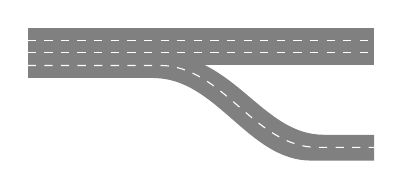
\begin{tikzpicture}[scale=.08]
\path[use as bounding box] (15,16.9) rectangle (70,38);
\fill[gray] (15,30) rectangle (38,38);
\fill[gray] (37.8,32) rectangle (70,38);
\fill[gray] (35,30) .. controls +(10,0) and (50,16.9) .. (60,16.9) -- (70,16.9) -- (70,21) -- (62,21) .. controls (52,21) and (48,34) .. (35,34);
\draw[dashed, white] (15,32) -- (36,32) .. controls +(10,0) and (51,19) .. (61,19) -- (70,19);
\draw[dashed, white] (15,34) -- (70,34);
\draw[dashed, white] (15,36) -- (70,36);
  \end{tikzpicture}  

&
  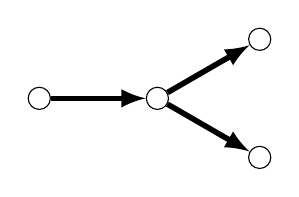
\begin{tikzpicture}[scale=1.5]
    \node[junc] (d) at (-1,0) {};
    \node[junc] (a) at (0,0) {};
    \node[junc] (b) at (30:1) {};
    \node[junc] (c) at (-30:1) {};
    \draw[link] (a) --node[above]{} (b);
    \draw[link] (a) --node[below]{} (c);
    \draw[link] (d) -- node[above, pos=.3]{} (a);
  \end{tikzpicture}
\end{tabular}
\caption{A diverging junction with one incoming link and two outgoing links as on a freeway (left) and schematically (right). When traffic flow is assumed to obey the \emph{first-in-first-out} (FIFO) property, congestion on link 2 (resp. 3) impedes flow to link 3 (resp. 2) whereas in a non-FIFO flow model, the flow from link 1 to link 2 (resp. link 3) is independent of the congestion on link 3 (resp. 2). For the FIFO case, if complete congestion on one outgoing link completely impedes the outgoing flow from link 1, the node model at the diverging junction is said to be \emph{full FIFO}, otherwise it is a \emph{partial FIFO} model.}
\label{fig:div}
\end{figure}

\section{Network Flow Model}
\label{sec:network-flow-model}
A traffic flow network consists of a directed graph  with \emph{junctions} or \emph{nodes}  and \emph{links} .   Let  and  denote the head and tail junction of link , respectively, where we assume , \emph{i.e.}, no self-loops. Traffic flows from  to . 

For each , we denote by  the set of input links to node  and by  the set of output links, \emph{i.e.},  

For each , we denote by  the set of links immediately upstream of link , and by  the set of links immediately downstream of link . We say that links  and  are \emph{adjacent} if  and  and let  be the set of links adjacent to link . Thus





Each link  has state  evolving over time that is the density of vehicles on link . We denote the  state of the network by . Vehicles flow from link to link over time; the state-dependent flow of vehicles from link  to link  is denoted by . We assume  if  so that flow is allowed only between links connected via a junction.  Furthermore, vehicles flow to link  from outside the network at rate  and vehicles leave the network from link  at rate  so that


In Section \ref{sec:examples}, we suggest specific forms for , , and  based on phenomenological properties of traffic flow. 

\newcommand{\fF}{f^\textnormal{F}}
\newcommand{\fNF}{f^\textnormal{NF}}

We further assume that each  is decomposable as

where  is the flow from link  to link  that is subject to the FIFO phenomenon and  is the flow from link  to link  that is not subject to the FIFO phenomenon.

The following captures the fundamental properties of traffic flow networks.
\begin{assum}
\label{assum:main}
For all , the functions , ,  are locally Lipschitz continuous. For all  where the given derivative exists,

\noindent \textbf{External flows:}
  \begin{enumerate}[label={(A\arabic*)},labelindent=*,leftmargin=*]
\item\label{eq:44}
  for all ,\\
\item \label{eq:44-2}    for all .
  \end{enumerate}
Interpretation:
  \begin{itemize}[leftmargin=*]
\item \ref{eq:44}: For any , increasing the density on link  can only increase the exogenous flow into link . For example, congestion on link  of the network causes vehicles that wish to enter the network to reroute and enter at link .
\item \ref{eq:44-2}: For any , increasing the density on link  can only decrease the flow that exits the network from link . For example, downstream congestion on link  impedes the outflow of vehicles via an offramp on link . 
  \end{itemize}
\noindent \textbf{Local dependence:}
\begin{enumerate}[label={(A\arabic*)},labelindent=*,leftmargin=*]
\setcounter{enumi}{2}
\item \label{eq:44-3}   for all  such that \\,
\item \label{eq:44-4}   for all  such that  \\ .
  \end{enumerate}
Interpretation:
\begin{itemize}[leftmargin=*]
\item \ref{eq:44-3} and \ref{eq:44-4}: The flow rate from link  to link  through some junction  is instantaneously affected by the change in density of vehicles on link  only if  is incoming or outgoing of junction .
\end{itemize}

\noindent \textbf{Net incoming and outgoing flows:}
\begin{enumerate}[label={(A\arabic*)},labelindent=*,leftmargin=*,itemsep=2pt]
\setcounter{enumi}{4}
\item \label{eq:44-7}  for all  such that ,
\item \label{eq:44-72}  for all  such that ,
\item \label{eq:44-8}   for all  such that .
  \end{enumerate}
Interpretation:
\begin{itemize}[leftmargin=*]
\item \ref{eq:44-7} and \ref{eq:44-72}: For any link  immediately upstream of link  (that is, ), increasing the density of vehicles on link  cannot decrease the net incoming FIFO or non-FIFO flow to link .
\item \ref{eq:44-8}: For any link  incoming or outgoing from junction , increasing the density of vehicles on link  cannot increase the net outgoing flow from link .
\end{itemize}
\noindent \textbf{FIFO and non-FIFO flows:}
\begin{enumerate}[label={(A\arabic*)},labelindent=*,leftmargin=*]
\setcounter{enumi}{7}
\item \label{eq:44-5}  for all ,
\item \label{eq:44-6} , for all .
  \end{enumerate}
Interpretation:
\begin{itemize}[leftmargin=*]
\item \ref{eq:44-5}: For any link  adjacent to link , increasing the density of link  can only increase the non-FIFO flow from an upstream link  to . This may occur if, \emph{e.g.}, vehicles reroute to avoid increased congestion on link .
\item \ref{eq:44-6}: For any link  adjacent to link , increasing the density of link  can only decrease the FIFO flow from an upstream link  to link . This captures the fundamental feature of FIFO flow whereby congestion on link  blocks access to link .
\end{itemize}
\end{assum}


Requirements \ref{eq:44}--\ref{eq:44-8} are standard for traffic flow networks. The requirement \ref{eq:44-5} is found in, \emph{e.g.}, \cite[Definition 2]{Como:2015ne} where it is used to establish monotonicity for non-FIFO policies. Requirement \ref{eq:44-6} captures the FIFO phenomenon.





\section{Mixed Monotonicity of Traffic Flow}
\label{sec:mixed-monot-traff}
\begin{definition}[Mixed Monotone]
\label{def:cwmm}
The system ,  where  has convex interior and  is locally Lipschitz is \emph{mixed monotone} if there exists a locally Lipschitz continuous function  satisfying:
\begin{enumerate}
\item  for all ,\\
\item  for all  and all   whenever the derivative exists,\\
\item  for all  and all   whenever the derivative exists.
\end{enumerate}
The function  is called a \emph{decomposition function} for the system.
\end{definition}


Let  be mixed monotone with decomposition function  and consider the dynamical system

The symmetry implies that if  is a trajectory of \eqref{eq:9}--\eqref{eq:9-2}, then  is also a trajectory.  Furthermore, observe that  is an invariant subspace of \eqref{eq:9}--\eqref{eq:9-2} and trajectories contained within this subspace correspond to (two copies of) trajectories of the original system , thus we refer to \eqref{eq:9}--\eqref{eq:9-2} as the \emph{embedding} system.


The importance of mixed monotonicity lies in the observation that the induced embedding system is monotone with respect to the partial order induced by the orthant , that is, \eqref{eq:9}--\eqref{eq:9-2}  is monotone with respect to the partial order  defined by  if and only if  and . This observation allows the powerful tools available for monotone systems to be applied to mixed monotone systems. For example, global convergence for \eqref{eq:9}--\eqref{eq:9-2} implies global convergence of the mixed monotone system . In Section \ref{sec:example}, we apply this technique to prove asymptotic convergence of the example in Figure \ref{fig:div}.


\begin{thm}
\label{thm:MM}
The traffic flow network model \eqref{eq:42} satisfying Assumption \ref{assum:main} is mixed monotone.
\end{thm}
\begin{proof}
  We construct an appropriate decomposition function . For each , let 

be defined elementwise as

Define 

and let . Then  given in \eqref{eq:42}--\eqref{eq:42-2} for all .
We next show

To this end, we show

which, combined with \ref{eq:44} and \ref{eq:44-2} of Assumption \ref{assum:main}, proves \eqref{eq:59}.  We have that \eqref{eq:60-2} holds for all  with  by \ref{eq:44-8}, and \ref{eq:44-3}--\ref{eq:44-4} ensures that \eqref{eq:60-2} holds with equality for all . For , \eqref{eq:60} holds from \ref{eq:44-7} and \ref{eq:44-72}. For , we have  for all  by \eqref{eq:56}, and  by \ref{eq:44-5}, satisfying \eqref{eq:60}. For , we have \eqref{eq:60} holds with equality by \ref{eq:44-3}--\ref{eq:44-4}.

We now show

We have that \eqref{eq:61} holds trivially for all  by \eqref{eq:56}. For , we have

where the inequality follows by \ref{eq:44-6}.
\end{proof}


We remark that a sufficient condition for mixed monotonicity of  is for each off-diagonal entry of the Jacobian matrix  to not change sign over the domain , that is, either  for all   or  for all  for all . This condition is proved for the discrete-time case in \cite{Coogan:2014ty} and the proof for the continuous-time case is similar. In general, partial FIFO models do not satisfy this condition; this is attributable to the different sign conditions in \ref{eq:44-5} and \ref{eq:44-6} whereby an increase on some link  may increase the non-FIFO flow to link  and decrease the FIFO flow to link . Thus we require a different construction for the decomposition function as shown in the proof of Theorem \ref{thm:MM}. 

We further observe that standard monotonicity is often generalized to partial orders induced by arbitrary orthants of  \cite{Angeli:2003fv}, and one may wonder if mixed monotonicity for traffic networks is equivalent to this generalization. As observed in \cite{Coogan:2015mz}, it is not difficult to construct traffic network topologies that are not monotone with respect to any orthant order, thus mixed monotonicity is strictly more general.










\section{Examples Of Models Satisfying Assumption \ref{assum:main}}
\label{sec:examples}


We now present several related examples satisfying \ref{eq:44}--\ref{eq:44-6} based on the \emph{supply} and \emph{demand} concept of traffic flow. We assume each link  possesses a \emph{jam density}  such that  for all time and thus . We further assume each link possesses a state-dependent \emph{demand} function  and a state-dependent \emph{supply} function  satisfying:
\begin{assum}
\label{assum:2}
  For each :
  \begin{itemize}
  \item The demand function  is strictly increasing and Lipschitz continuous with .
  \item The supply function  is strictly decreasing and Lipschitz continuous with .
  \end{itemize}
\end{assum}

The demand of a link is interpreted as the maximum outflow of the link, and the supply of a link is interpreted as the maximum inflow of the link. 

Let , that is,  is the set of links for which there are no upstream links. We assume exogenous traffic enters the network only through  so that


For each , we assume there exists a constant exogenous inflow demand  such that


We further assume that  is a fixed fraction  of the total outflow from link  if there are any links downstream of , otherwise  is equal to the demand of link . That is, for all ,

where  for each  such that .


Finally, we assume there exist fixed turn ratios  for each  with  that describe how vehicles route through the network. The role of these turn ratios is made explicit subsequently, but the interpretation is that  is the fraction of the upstream demand that is bound for link . 



 It remains to characterize  for all .

\begin{example}[non-FIFO]
\label{ex:1}
For all , let
  
Let  for all  and let

\end{example}


\begin{example}[Full FIFO]
\label{ex:2}
For all , let
  
Let  for all  and let

\end{example}

\begin{example}[Convex combination of non-FIFO and full FIFO]
\label{ex:3}
  Let  be given as in \eqref{eq:45} and let  be given as in \eqref{eq:45-2}. Suppose there exists  for all , and let
  
\end{example}

Example \ref{ex:3} is proposed in  \cite[Example 4]{Lovisari:2014qv} and is a natural extension of the ideas in Examples \ref{ex:1} and \ref{ex:2}, however it exhibits the following property: it is possible for  yet , that is, the supply of link  restricts the flow to link , yet the total inflow of link  is less than this supply. This property may be undesirable, depending on the specific phenomena which the node model is desired to capture. We now suggest an alternative partial FIFO model. To fix ideas, we assume that each diverging junction has exactly one incoming link, that is,

This is not too restrictive as we can model a general diverging junction as a merging node and a node satisfying \eqref{eq:6}.

\newcommand{\thetaF}{\theta^\textnormal{F}}
\begin{example}[Shared and exclusive lanes for a partial FIFO model]
\label{ex:4}
Assume \eqref{eq:6} holds. We consider  for each  representing the degree of influence on link  of the FIFO restriction at the intersection so that  is the fraction of traffic bound for link  that is subject to a FIFO restriction and  is the fraction of traffic bound for link  that is not subject to a FIFO restriction. For example,  is the fraction of lanes at the diverging junction exclusively bound for link  and  is the fraction of lanes that are shared among all outgoing links. 

Whenever , we assume  without loss of generality.
Let  be given as in \eqref{eq:45-2} for all .
For  such that , let  be the unique link such that  (uniqueness is guaranteed by \eqref{eq:6}), and let

For  such that , we have that  so that

\end{example}


We extend Example \ref{ex:4} to the case where there are multiple sets of interacting outgoing links that result in a collection of FIFO restrictions.
\newcommand{\F}{\mathcal{F}}
\begin{example}
  \label{ex:5}
Assume \eqref{eq:6} holds. For each  with , let  be a collection of subsets of  so that each ,  is a set links which are mutually governed by a FIFO restriction. When , we assume .

 For  and , let  represent the degree of influence on link  of the FIFO restriction set . We make the following assumptions:

Define

For all  such that , define

where  is the unique upstream link such that .

For  such that , let  be the unique link such that , and let

For  such that , we again let

where  is as given in \eqref{eq:45-2}.
\end{example}
Taking  for all , we see that Example \ref{ex:4} is a special case of Example \ref{ex:5}.

All the examples above satisfy, for all ,


If we further assume that  and 

for all  such that , we have that, for all ,




\begin{prop}
\label{sec:examples-1}
  Examples \ref{ex:1}--\ref{ex:5} satisfy Assumption \ref{assum:main}.
\end{prop}
\begin{proof}

It follows straightforwardly from results in \cite{Lovisari:2014qv} that the conditions of Assumption \ref{assum:main} hold for Example \ref{ex:1}, and, similarly, it follows from results in \cite{Coogan:2015mz} that the assumption holds for Example \ref{ex:2}. From Example 1 and Example 2, the assumption immediately holds for Example \ref{ex:3}. We now show that Example \ref{ex:5} satisfies Assumption \ref{assum:main}, from which it follows that also Example \ref{ex:4} satisfies Assumption \ref{assum:main} because Example \ref{ex:4} is a special case of Example \ref{ex:5}. To that end, we now prove each condition \ref{eq:44}--\ref{eq:44-6} for Example 5.



\begin{itemize}[leftmargin=*]
\item    (Condition \ref{eq:44}).  Follows trivially from \eqref{eq:39} and \eqref{eq:40}.
    \item    (Condition \ref{eq:44-2}). Follows from \eqref{eq:41} and Condition \ref{eq:44-8}, proved below, as well as Conditions \ref{eq:44-3} and \ref{eq:44-4}, proved below.
    \item    (Conditions \ref{eq:44-3} and \ref{eq:44-4}). Follows immediately from the fact that for all  and all ,  and  are only functions of  for  and  for  and from \eqref{eq:8-2}.
 \item    (Conditions \ref{eq:44-7} and \ref{eq:44-72}). 
Consider . If , then  by \eqref{eq:6} and

and thus \ref{eq:44-7} and \ref{eq:44-72} hold. 

Now suppose  and let  so that

We have 

and thus \ref{eq:44-7} holds by \eqref{eq:8} and \eqref{eq:20}.

Still supposing  with , consider now Condition \ref{eq:44-72}. The only possibility for which this condition would not hold is if  is the minimizer in \eqref{eq:8-2} and . But

only if  for some  for which  on some neighborhood of  so that, in particular, . In this case, since , we have that

\emph{i.e.},  is the minimizer in \eqref{eq:8-2} and thus \ref{eq:44-72} holds.

    \item    (Condition \ref{eq:44-8}). 
 Suppose  is such that  and let . Consider . Then

Since  for all  with , and , \ref{eq:44-8} holds.

 Now suppose  so that , and let . 
From \eqref{eq:8}--\eqref{eq:8-2}, for all  we have

Consider some . Then 

so that  for all , and

for all . From \eqref{eq:17}, we have that  for all  so that \ref{eq:44-8} holds. Finally, when , condition \ref{eq:44-8} holds trivially for all .
   
    \item    (Condition \ref{eq:44-5}). Follows from Condition \ref{eq:44-6} below and \eqref{eq:8-2}. 
    \item    (Condition \ref{eq:44-6}).  Follows from \eqref{eq:8}, \eqref{eq:16}, and the fact that  for all .
\end{itemize}
\end{proof}





\section{Analysis from Mixed Monotonicity: Diverging Junction}
\label{sec:example}














We return to the example of Figure \ref{fig:div} and suppose the diverging junction obeys the dynamics given in Example \ref{ex:4} of Section \ref{sec:examples}. We assume for all 

where  corresponds to the lane configuration in Figure \ref{fig:div}, , turn ratios  indicates that most of the traffic is bound for link 2, and  indicates that link 3 is strongly affected by the FIFO restriction but link 2 is not. We assume  is the desired inflow to link 1. 

Let  be the trajectory of the symmetric system \eqref{eq:9}--\eqref{eq:9-2} with initial condition  and  where  is constructed as in the proof of Theorem \ref{thm:MM}. We have

that is,  where we recall that  is the partial order induced by the orthant . It follows that  is increasing with respect to  \cite[Ch. 3, Prop. 2.1]{Smith:2008fk}, and thus converges to an equilibrium . By symmetry, we have that also  is a trajectory of \eqref{eq:9}--\eqref{eq:9-2} converging to . If , then we must have that  is an equilibrium of the traffic flow dynamics defined by \eqref{eq:42}--\eqref{eq:42-2}. Furthermore, because the symmetric system is monotone with respect to , we must have that all trajectories of \eqref{eq:7}--\eqref{eq:7-2} converge to , which in turn implies that  is globally attractive for the traffic flow dynamics.



 In the top row of Figure \ref{fig:plots}, we plot the demand and supply curves given in \eqref{eq:7}--\eqref{eq:7-2}. We establish global convergence by verifying that an equilibrium  of \eqref{eq:9}--\eqref{eq:9-2} satisfies . The particular form of the supply and demand functions does not affect the qualitative behavior and \eqref{eq:7}--\eqref{eq:7-2} is chosen to be illustrative. The bottom row of Figure \ref{fig:plots} shows the trajectories  and  projected to the -plane for each .
 \begin{figure}
   \centering
   \begin{tabular}{@{}c@{}@{}c@{}@{}c@{}}
\includegraphics[scale=.45,clip=true,trim=.05in 0.1in 0in 0.1in]{sim_ds_0}&     \includegraphics[scale=.45,clip=true,trim=.05in 0.1in 0in 0.1in]{sim_ds_1}&  \includegraphics[scale=.45,clip=true,trim=.05in 0.1in 0in .1in]{sim_ds_2}\-3pt]
 \includegraphics[scale=.45,clip=true,trim=.05in 0.1in 0in 0.1in]{sim_xy_0}&\includegraphics[scale=.45,clip=true,trim=.05in 0.1in 0in .1in]{sim_xy_1}&\includegraphics[scale=.45,clip=true,trim=.05in 0.1in 0in 0.1in]{sim_xy_2}\\
\multicolumn{3}{c}{\includegraphics[scale=.45]{legend}}
   \end{tabular}

\caption{\noindent \textbf{(top)} Supply and demand curves for each link  of the diverging junction show in Figure \ref{fig:div} for the example in Section \ref{sec:example}. \textbf{(bottom)} Trajectories of the corresponding embedding system \eqref{eq:9}--\eqref{eq:9-2}. Mixed monotonicity ensures the embedding system is monotone with respect to the orthant . Convergence of the symmetric extreme trajectories  and  for ,  implies global convergence. The traffic flow dynamics are captured on a lower dimensional subspace of the embedding system, indicated by the dotted line.}
   \label{fig:plots}
 \end{figure}

\section{Conclusions}
\label{sec:conclusions}
We have proposed a general model for traffic flow networks that encompasses existing models and allows for a relaxed FIFO assumption at diverging junctions. We have shown that this general model is mixed monotone and have demonstrated how mixed monotonicity is used for system analysis such  as establishing global convergence. In future work, we will use mixed monotonicity to characterize traffic flow behavior for, \emph{e.g.}, cyclic networks, networks with excess demand, or networks with time-varying demand.

\section*{Acknowledgements}
The authors thank Gabriel Gomes and Giacomo Como for fruitful discussion regarding the limitations of non-FIFO and full FIFO traffic flow models.


\bibliographystyle{ieeetr}
\begin{thebibliography}{10}

\bibitem{Lovisari:2014qv}
E.~Lovisari, G.~Como, A.~Rantzer, and K.~Savla, ``Stability analysis and
  control synthesis for dynamical transportation networks,'' {\em arXiv
  preprint arXiv:1410.5956}, 2014.

\bibitem{Hirsch:1985fk}
M.~W. Hirsch, ``Systems of differential equations that are competitive or
  cooperative {II}: Convergence almost everywhere,'' {\em SIAM Journal on
  Mathematical Analysis}, vol.~16, no.~3, pp.~423--439, 1985.

\bibitem{Smith:2008fk}
H.~L. Smith, {\em Monotone dynamical systems: {A}n introduction to the theory
  of competitive and cooperative systems}.
\newblock American Mathematical Society, 1995.

\bibitem{Coogan:2015mz}
S.~Coogan and M.~Arcak, ``Stability of traffic flow networks with a polytree
  topology,'' {\em Automatica}, vol.~66, pp.~246--253, April 2016.

\bibitem{Smith:2008rr}
H.~Smith, ``Global stability for mixed monotone systems,'' {\em Journal of
  Difference Equations and Applications}, vol.~14, no.~10-11, pp.~1159--1164,
  2008.

\bibitem{Coogan:2014ty}
S.~Coogan and M.~Arcak, ``Efficient finite abstraction of mixed monotone
  systems,'' in {\em Proceedings of the 18th International Conference on Hybrid
  Systems: Computation and Control}, pp.~58--67, 2015.

\bibitem{Cassidy2002563}
M.~J. Cassidy, S.~B. Anani, and J.~M. Haigwood, ``Study of freeway traffic near
  an off-ramp,'' {\em Transportation Research Part A: Policy and Practice},
  vol.~36, no.~6, pp.~563--572, 2002.

\bibitem{Munoz:2002qv}
J.~C. Munoz and C.~F. Daganzo, ``The bottleneck mechanism of a freeway
  diverge,'' {\em Transportation Research Part A: Policy and Practice},
  vol.~36, no.~6, pp.~483--505, 2002.

\bibitem{wrightetal16a}
M.~Wright, G.~Gomes, R.~Horowitz, and A.~A. Kurzhanskiy, ``On node and route
  choice models for high-dimensional road networks,'' 2016.
\newblock arXiv:1601.01054.

\bibitem{bliemer07}
M.~Bliemer, ``Dynamic queueing and spillback in an analytical multiclass
  dynamic network loading model,'' {\em Transportation Research Record},
  vol.~2029, pp.~14--21, 2007.

\bibitem{shiomi2015}
Y.~Shiomi, T.~Taniguchi, N.~Uno, H.~Shimamoto, and T.~Nakamura, ``Multilane
  first-order traffic flow model with endogenous representation of lane-flow
  equilibrium,'' {\em Transportation Research Part C: Emerging Technologies},
  vol.~59, pp.~198--215, 2015.

\bibitem{Como:2015ne}
G.~Como, E.~Lovisari, and K.~Savla, ``Throughput optimality and overload
  behavior of dynamical flow networks under monotone distributed routing,''
  {\em IEEE Transactions on Control of Network Systems}, vol.~2, pp.~57--67,
  March 2015.

\bibitem{Angeli:2003fv}
D.~Angeli and E.~Sontag, ``Monotone control systems,'' {\em IEEE Transactions
  on Automatic Control}, vol.~48, no.~10, pp.~1684--1698, 2003.

\end{thebibliography}
 

\end{document}